\documentclass[letterpaper,10pt]{article}

\usepackage{enumitem}
\usepackage{titling}
\usepackage{listings,listings-rust}
\usepackage{url}
\usepackage{soul}
\usepackage{hyperref}
\usepackage{setspace}
\usepackage{subfig}
\usepackage{sectsty}
\usepackage{pdfpages}
\usepackage{colortbl}
\usepackage{multirow}
\usepackage{multicol}
\usepackage{relsize}
\usepackage{amsmath}
\usepackage{wasysym}
\usepackage{fancyvrb}
\usepackage[yyyymmdd]{datetime}
\usepackage{amsmath,amssymb,amsthm,graphicx,xspace}
\usepackage[titlenotnumbered,noend,noline]{algorithm2e}
\usepackage[compact]{titlesec}
\usepackage{XCharter}
\usepackage[T1]{fontenc}
\usepackage[scaled]{beramono}
\usepackage[normalem]{ulem}
\usepackage{booktabs}
\usepackage{tikz}
\usetikzlibrary{arrows.meta,automata,shapes,trees,matrix,chains,scopes,positioning,calc,decorations.pathreplacing}
\tikzstyle{block} = [rectangle, draw, fill=blue!20, 
    text width=2.5em, text centered, rounded corners, minimum height=2em]
\tikzstyle{bw} = [rectangle, draw, fill=blue!20, 
    text width=4em, text centered, rounded corners, minimum height=2em]

\definecolor{namerow}{cmyk}{.40,.40,.40,.40}
\definecolor{namecol}{cmyk}{.40,.40,.40,.40}
\renewcommand{\dateseparator}{-}

\let\LaTeXtitle\title
\renewcommand{\title}[1]{\LaTeXtitle{\textsf{#1}}}

\lstset{basicstyle=\footnotesize\ttfamily,breaklines=true}

\newcommand{\CPP}{C\nolinebreak\hspace{-.05em}\raisebox{.4ex}{\tiny\bf +}\nolinebreak\hspace{-.10em}\raisebox{.4ex}{\tiny\bf +}}
\def\CPP{{C\nolinebreak[4]\hspace{-.05em}\raisebox{.4ex}{\tiny\bf ++}}}

\newcommand{\handout}[5]{
  \noindent
  \begin{center}
  \framebox{
    \vbox{
      \hbox to 5.78in { {\bf ECE459: Programming for Performance } \hfill #2 }
      \vspace{4mm}
      \hbox to 5.78in { {\Large \hfill #4  \hfill} }
      \vspace{2mm}
      \hbox to 5.78in { {\em #3 \hfill \today} }
    }
  }
  \end{center}
  \vspace*{4mm}
}

\newcommand{\lecture}[3]{\handout{#1}{#2}{#3}{Lecture#1}}
\newcommand{\tuple}[1]{\ensuremath{\left\langle #1 \right\rangle}\xspace}

\addtolength{\oddsidemargin}{-1.000in}
\addtolength{\evensidemargin}{-0.500in}
\addtolength{\textwidth}{2.0in}
\addtolength{\topmargin}{-1.000in}
\addtolength{\textheight}{1.75in}
\addtolength{\parskip}{\baselineskip}
\setlength{\parindent}{0in}
\renewcommand{\baselinestretch}{1.5}
\newcommand{\term}{Winter 2020}

\singlespace


\begin{document}

\lecture{27 --- Liar, Liar and Memory Profiling}{\term}{Patrick Lam \& Jeff Zarnett}

I was thinking today about how humans are quite adept at building and
using tools (though not
unique\footnote{https://www.rnz.co.nz/news/national/366747/clever-kea-using-tools-to-raid-traps}). Profilers
are useful tools, but they can mislead you.  If you understand how
profilers work, you can avoid being misled.

As we've been saying this week, there are sampling-based and instrumentation-based profilers.
The tl;dr is that a sampling-based profiler can miss things, while an instrumentation-based
profiler distorts the system under observation.

Visually, sampling-based profiling can do this:
\begin{center}
	\url{https://www.youtube.com/watch?v=jQDjJRYmeWg}
\end{center}

The video's not fake; it's a real helicopter and it's really flying. What's happening, however, is that the camera is taking images at some multiple of the frequency of the blade rotation speed so it gives the illusion that the blades are not spinning at all. This is a sampling problem, and you see the same problem in car commercials on TV where it looks like the wheels are spinning backwards. They're not, but the sampling effect of the camera can make it look that way.

The main assumptions underlying sampling are that samples are ``random'' and that the sample distribution approximates the actual time-spent distribution\footnote{Lifted from ``Profilers are Lying Hobbitses'', \url{https://www.infoq.com/presentations/profilers-hotspots-bottlenecks/}, which talks about profiling for JVMs.}.

\section*{Lies from Metrics}
While app-specific metrics can lie too, mostly we'll talk about CPU
perf counters today.
In particular, we're going to look at two types of sampling-based lies.

The reference for the first type of lie is a blog post by Paul Khuong~\cite{metrics}.

This goes back to {\tt mfence}, which we've seen before. It is used, for instance, in
spinlock implementations. Khuong found that his profiles said that spinlocking didn't take much time.
But empirically: eliminating spinlocks = better than expected! Hmm.

The next step is (as we do in this course) to create microbenchmarks to better understand what's
going on. The microbenchmark contained memory accesses to uncached locations, or computations,
surrounded by store pairs/mfence/locks. He used perf to evaluate the impact of mfence vs lock.
You'll recall that perf is sampling-based and records how often the CPU is found executing each
instruction.

{\scriptsize
\begin{lstlisting}
# for locks:
$ perf annotate -s cache_misses
[...]
    0.06 :        4006b0:       and    %rdx,%r10
    0.00 :        4006b3:       add    $0x1,%r9
    ;; random (out of last level cache) read
    0.00 :        4006b7:       mov    (%rsi,%r10,8),%rbp
   30.37 :        4006bb:       mov    %rcx,%r10
    ;; foo is cached, to simulate our internal lock
    0.12 :        4006be:       mov    %r9,0x200fbb(%rip)
    0.00 :        4006c5:       shl    $0x17,%r10
    [... Skipping arithmetic with < 1% weight in the profile]
    ;; locked increment of an in-cache "lock" byte
    1.00 :        4006e7:       lock incb 0x200d92(%rip)
   21.57 :        4006ee:       add    $0x1,%rax
    [...]
    ;; random out of cache read
    0.00 :        400704:       xor    (%rsi,%r10,8),%rbp
   21.99 :        400708:       xor    %r9,%r8
    [...]
    ;; locked in-cache decrement
    0.00 :        400729:       lock decb 0x200d50(%rip)
   18.61 :        400730:       add    $0x1,%rax
    [...]
    0.92 :        400755:       jne    4006b0 <cache_misses+0x30>
\end{lstlisting}
}

We can see that in the lock situation, reads take 30 + 22 = 52\% of runtime,
while locks take 19 + 21 = 40\% of runtime.

{\scriptsize
\begin{lstlisting}
# for mfence:
$ perf annotate -s cache_misses
[...]
    0.00 :        4006b0:       and    %rdx,%r10
    0.00 :        4006b3:       add    $0x1,%r9
    ;; random read
    0.00 :        4006b7:       mov    (%rsi,%r10,8),%rbp
   42.04 :        4006bb:       mov    %rcx,%r10
    ;; store to cached memory (lock word)
    0.00 :        4006be:       mov    %r9,0x200fbb(%rip)
    [...]
    0.20 :        4006e7:       mfence 
    5.26 :        4006ea:       add    $0x1,%rax
    [...]
    ;; random read
    0.19 :        400700:       xor    (%rsi,%r10,8),%rbp
   43.13 :        400704:       xor    %r9,%r8
    [...]
    0.00 :        400725:       mfence 
    4.96 :        400728:       add    $0x1,%rax
    0.92 :        40072c:       add    $0x1,%rax
    [...]
    0.36 :        40074d:       jne    4006b0 <cache_misses+0x30>
\end{lstlisting}
}
Looks like the reads take 85\% of runtime,
while the mfence takes 15\% of runtime.

Metrics lie, though, and when you focus on the metrics as opposed to what you
actually care about, it's easy to be led astray.

In this case, what we actually care about is the total \# of cycles.

    \begin{tabular}{lr}
    No atomic/fence:& 2.81e9 cycles\\
    lock inc/dec: & 3.66e9 cycles\\
    mfence: & 19.60e9 cycles
    \end{tabular}

That 15\% number is a total lie.
Profilers, even using CPU expense counts, drastically underestimate the impact of mfence,
and overestimate the impact of locks.

This is because mfence causes a pipeline flush, and the resulting 
costs get attributed to instructions being flushed, not to the mfence itself. In other
words, mfence makes other instructions run more slowly, which camouflages its own effect
on the overall performance.


\section*{The Long Tail}

The other type of lie that sampling can hide is the one where infrequent long tails are hidden in averages.
Our source here is the blog post by Dan Luu~\cite{perf-tracing}. Suppose we have a task that's going to get distributed over multiple computers (like a search). If we look at the latency distribution, the problem is mostly that we see a long tail of events and when we are doing a computation or search where we need all the results, we can only go as the slowest step. Let's take a look at a histogram of disk read latencies, where we are performing a 64 kB read, also from that source:

\begin{center}
	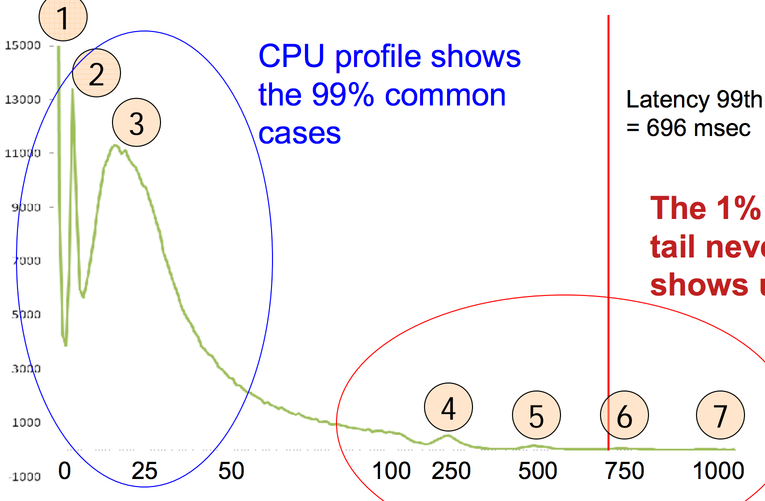
\includegraphics[width=0.5\textwidth]{images/disk_tail.png}
\end{center}

Let's break it down. Peak 1 corresponds to something cached in RAM---best case scenario. Peak 2 is at around 3ms, which is too fast for spinning and seeking magnetic hard disks, but it's fast enough for reading something from the disk cache via the PCI-Express interface. Peak 3 is obviously disk seek and read times, around 25ms. 

These numbers don't look terrible, except for the fact that we have peaks at 250, 500, 750, and 1000 ms and the 99th percentile is some 696ms which is a very, very long time. Sampling profilers are not very good at finding these things, because they throw everything into various buckets and therefore we get averages. The averages are misleading, though, because we have these weird outliers that take dramatically longer. Averages are nice as long as our data is also reasonably ``nice''.

So what actually happened? Well, from~\cite{perf-tracing}: The investigator found out that the cause was kernel throttling of the CPU for processes that went beyond their usage quota. To enforce the quota, the kernel puts all of the relevant threads to sleep until the next multiple of a quarter second. When the quarter-second hand of the clock rolls around, it wakes up all the threads, and if those threads are still using too much CPU, the threads get put back to sleep for another quarter second. The phase change out of this mode happens when, by happenstance, there aren't too many requests in a quarter second interval and the kernel stops throttling the threads. After finding the cause, an engineer found that this was happening on 25\% of disk servers at Google, for an average of half an hour a day, with periods of high latency as long as 23 hours. This had been happening for three years.

Further limitations of sampling profilers emerge, as demonstrated in this graph, also from~\cite{perf-tracing}, showing the data we get out of our sampling profiler if we take a look at Lucene (a search indexer):

\begin{center}
	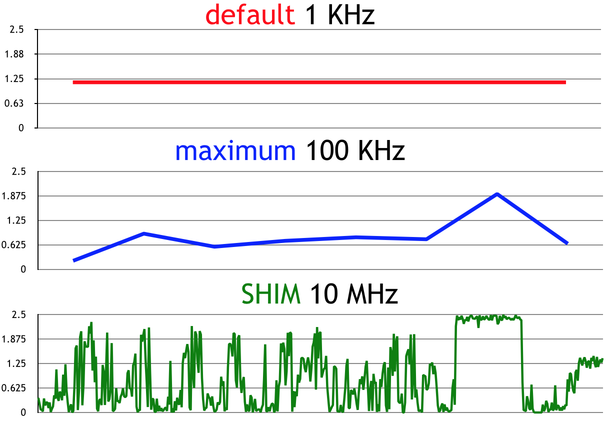
\includegraphics[width=0.3\textwidth]{images/perf-sample.png}
\end{center}

So at the default sampling interval for perf we see\ldots nothing interesting whatsoever. If we bump up to the max sampling frequency of perf, we get a moderately more interesting graph, but not much. If we use a different tool and can sample at a dramatically higher rate, then we end up with something way more useful. So we're left to wonder why does perf sample so infrequently, and how does SHIM get around this?

Well, for one thing, perf samples are done with interrupts. Processing interrupts takes a fair amount of time and if you crank up the rate of interrupts, before long, you are spending all your time handling the interrupts rather than doing useful work. So sampling tools usually don't interrupt the program too often. SHIM gets around this by being more invasive---it instruments the program, adding some periodically executed code that puts information out whenever there is an appropriate event (e.g., function return). This produces a bunch of data which can be dealt with later to produce something useful.

This instrumentation-based approach is more expensive in general, but note that DTrace\footnote{Note also the comment in the blog post: ``Yes, that includes dtrace, which I'm calling out in particular because any time you have one of these discussions, a dtrace troll will come along to say that dtrace has supported that for years. It's like the common lisp of trace tools, in terms of community trolling.''} and Nethercote's counts tool (discussed in L25) also enable custom instrumentation of select events. 

\section*{Lies from Counters}
This is fairly niche, but Rust compiler hackers were trying to include
support for hardware performance counters (what perf reports) because
{\tt -Z self-profile} data was too noisy\footnote{Full story, in gory
detail,
at \url{https://hackmd.io/sH315lO2RuicY-SEt7ynGA?view}.}. Counters
are, for instance, faster than measuring time and way (i.e. 5 orders of magnitude) more deterministic.

To make counters as deterministic as possible:
\begin{itemize}[noitemsep]
\item disable Address Space Layout Randomization (randomized pointer addresses affect hash layouts);
\item subtract time spent processing interrupts (IRQs);
\item profile one thread only (if you can, in your context).
\end{itemize}
Fun fact. We talked about Spectre back in Lecture 7. Speculative execution comes up here too in terms of
counters being wrong. AMD speculates past atomics and then rolls back, but doesn't roll back perf counters.
Post-Spectre, there's a hidden model-specific register (``SpecLockMap'') that disables speculating past atomics, the kind of thing you would
want around to protect you against future things in that vein that someone might discover. Or, in better words than mine\footnote{\url{https://twitter.com/eddyb_r/status/1323587371703668742}}:

\begin{center}

\includegraphics{images/L27-eb-tweet.png}
\end{center}

\section*{Lies about Calling Context}
This part is somewhat outdated now, as it's a pretty specific technical problem that especially arises under the {\tt gprof} tool. It's still a good example of lying tools, though,
so I'll include a condensed version. Yossi Kreinin~\cite{lies} writes about it in more detail.

gprof uses two C standard-library functions: {\bf profil()} and {\bf mcount()}.

\vspace*{-1em}
\begin{itemize}[noitemsep]
\item {\bf profil()}: asks glibc to record which instruction 
  is currently executing (100$\times$/second).
\item {\bf mcount()}: records call graph edges; called by {\tt -pg} instrumentation.
\end{itemize}
\vspace*{-1em}

Hence, {\bf profil} information is statistical, while {\bf mcount}
information is exact.  gprof can draw unreliable inferences. If you have a method \texttt{easy} and a method \texttt{hard}, each of which is called once, and \texttt{hard} takes up almost all the CPU time,
gprof might divide total time by 2 and report bogus results.

The following results from gprof are suspect (among others):
\vspace*{-1em}
\begin{itemize}[noitemsep]
  \item contribution of children to parents;
  \item total runtime spent in self+children;
\end{itemize}
\vspace*{-1em}

\paragraph{When are call graph edges right?}
Two cases:
\vspace*{-1em}
    \begin{itemize}[noitemsep]
    \item functions with only one caller
      (e.g. {\tt f()} only called by {\tt g()}); or,
    \item functions which always take the same time to complete
      (e.g. {\tt rand()}).
    \end{itemize}
\vspace*{-1em}

On the other hand, results for any function whose running time depends on its inputs,
and which is called from multiple contexts, are sketchy.


Next, we'll talk about callgrind/KCacheGrind. Like our old friends memcheck, helgrind, and cachegrind, callgrind is part of valgrind, and runs the program under an x86 JIT.  KCacheGrind is a frontend to callgrind. callgrind gives better information, but imposes
more overhead.
KCacheGrind works properly on the earlier running example, but we can still deceive it with more complicated examples.

%% \paragraph{Summary.} We've seen that some profiler results are exact;
%% some results are sampled; and some results are interpolated. If you understand the tool, you understand where it can go
%% wrong. 

%% Understand your tools!


\paragraph{Overall summary.} We saw a bunch of lies today: calling-context lies and perf attribution
lies. To avoid being bitten by lies, remember to focus on the metric you actually care about,
and understand how your tools work.

\section*{Memory Profiling}

Thus far we have focused on CPU profiling. Other kinds of profiling got some mention, but they're not the only kind of profiling we can do. Memory profiling is also a thing, and specifically we're going to focus on heap profiling.

During Rustification, we dropped a bunch of valgrind content. Valgrind is a memory error and leak detection toolset that is invaluable when programming in \CPP. (In brief: valgrind is a just-in-time engine that reinterprets machine code and instruments it to find sketchy things.) In particular, the memory leaks that valgrind's memcheck tool detects are, for the most part, not possible in Rust unless you try pretty hard\footnote{You can still create cycles in refcounted objects or call \texttt{std::mem::forget} or etc.}---the friendly compiler protects you against them by automatically dropping things.

We're going to look at two kinds of memory profiling here, both part of valgrind. They can both occur in Rust, but it looks like the more common kind is when a lot of memory is allocated and then freed. More completely: ``places that cause excessive numbers of allocations; leaks; unused and under-used allocations; short-lived allocations; and allocations with inefficient data layouts''. valgrind's DHAT tool~\cite[Chapter~10]{valgrind} detects these.

The second kind of memory profiling addresses memory that memcheck reports as ``Still Reachable''. That is, things that remained allocated and still had pointers to them, but were not properly deallocated. Right, we care about them too, and for that we also want to do heap profiling. If we don't look after those things, we're just using more and more memory over time. That likely means more paging and the potential for running out of heap space altogether. Again, the memory isn't really lost, because we could free it.

\subsection*{DHAT}
DHAT tracks allocation points and what happens to them over a program's execution. An allocation point is a point in the program which allocates memory; in C that would be \texttt{malloc}. In Rust there are a bunch of ways to allocate memory, one being \texttt{Box::new}. It aggregates allocation points according to the program stack. Let's first look at a leaf node from the documentation.

\begin{verbatim}
AP 1.1.1.1/2 {
  Total:     31,460,928 bytes (2.32%, 1,565.9/Minstr) in 262,171 blocks (4.41%, 13.05/Minstr), 
     avg size 120 bytes, avg lifetime 986,406,885.05 instrs (4.91% of program duration)
  Max:       16,779,136 bytes in 65,543 blocks, avg size 256 bytes
  At t-gmax: 0 bytes (0%) in 0 blocks (0%), avg size 0 bytes
  At t-end:  0 bytes (0%) in 0 blocks (0%), avg size 0 bytes
  Reads:     5,964,704 bytes (0.11%, 296.88/Minstr), 0.19/byte
  Writes:    10,487,200 bytes (0.51%, 521.98/Minstr), 0.33/byte
  Allocated at {
    ^1: 0x95CACC9: alloc (alloc.rs:72)
      [omitted]
    ^7: 0x95CACC9: parse_token_trees_until_close_delim (tokentrees.rs:27)
    ^8: 0x95CACC9: syntax::parse::lexer::tokentrees::<impl syntax::parse::lexer::
                          StringReader<'a>>::parse_token_tree (tokentrees.rs:81)
    ^9: 0x95CAC39: parse_token_trees_until_close_delim (tokentrees.rs:26)
    ^10: 0x95CAC39: syntax::parse::lexer::tokentrees::<impl syntax::parse::lexer::
                          StringReader<'a>>::parse_token_tree (tokentrees.rs:81)
    #11: 0x95CAC39: parse_token_trees_until_close_delim (tokentrees.rs:26)
    #12: 0x95CAC39: syntax::parse::lexer::tokentrees::<impl syntax::parse::lexer::
                          StringReader<'a>>::parse_token_tree (tokentrees.rs:81)
  }
}
\end{verbatim}

We can see the program point corresponding to this allocation: line 81 of \texttt{tokentrees.rs}.
Furthermore, the most bytes alive at once from this site was 16,779,136: that was 65,543 instances of the
memory allocated here, almost all 256-byte blocks. In total, this allocation site was executed
262,171 times, accounting for 31,460,928 bytes. This information can tell us how important this
allocation site is compared to the entire execution we're inspecting. We can also see how long-lived
the blocks are: on average, a block allocated here lives 4.91\% of the program duration. If instead of
4.91\% we had 0.004\% and a large total, then the allocation point would be excessively transient and perhaps
a good candidate for pooling allocations.

The Reads and Writes lines tell us how often the allocated memory is actually used. In this case,
19\% of the bytes allocated here are ever read, and 33\% are written to. That seems like not many, but if it's something
like a vector that grows, you may not be able to do anything about that. This, however, doesn't look like a vector---you
could check it by looking at the code.

You might also get a super-useful Accesses line if all of the blocks allocated at a site are the same size.
That line tells you how many times each byte in the block was accessed. Zeros, written as dashes (-), are
parts of the block that are never accessed, useful for finding data alignment holes (and hence potential
inefficiencies).

\paragraph{Parents.} Going up the tree, DHAT tells you about all of the allocation points that share a call-stack
prefix. (The \verb+^+ before the number indicates that the line is copied from the parent; a \# indicates that the line is unique to
that node.)

A sibling of the example above would diverge at the call on line 10, not calling
\texttt{parse\_token\_trees\_until\_close\_delim} from line 81 of \texttt{tokentrees.rs}. At the parent, DHAT
reports results for that node and all of its children.

\subsection*{\st{Memory Profiling} Return to Asgard}
JZ generally found a way to talk about Valgrind in previous courses. But now, we're going to use its Massif tool. This is, obviously, a joke on ``massive'', combined with the name Sif, a Norse goddess associated with the earth (and in the Marvel movies, Shieldmaiden to Thor).

So what does Massif do? It will tell you about how much heap memory your program is using, and also how the situation got to be that way. So let's start with the example program from the documentation, badly translated by yours truly to non-idiomatic Rust~\cite{massif}:


\begin{lstlisting}[language=Rust]
fn g() {
    let a = Vec::<u8>::with_capacity(4000);
    std::mem::forget(a)
}

fn f() {
    let a = Vec::<u8>::with_capacity(2000);
    std::mem::forget(a);
    g()
}

fn main() {

    let mut a = Vec::with_capacity(10);
    for _i in 0..10 {
	a.push(Box::new([0;1000]))
    }
    f();
    g();
}
\end{lstlisting}


After we compile, run the command:
{\scriptsize
\begin{verbatim}
plam@amqui ~/c/p/l/l/L/alloc> valgrind --tool=massif target/debug/alloc
==406569== Massif, a heap profiler
==406569== Copyright (C) 2003-2017, and GNU GPL'd, by Nicholas Nethercote
==406569== Using Valgrind-3.16.1 and LibVEX; rerun with -h for copyright info
==406569== Command: target/debug/alloc
==406569== 
==406569== 
\end{verbatim}
}

Doesn't that look useful?! What happened? Your program executed slowly, as is always the case with any of the Valgrind toolset, but you don't get summary data on the console like we did with Valgrind or helgrind or cachegrind. Weird. What we got instead was the file \texttt{massif.out.406569} (matches the PID of whatever we ran). This file, which you can open up in your favourite text editor, is not especially human readable, but it's not incomprehensible like the output from cachegrind (``Aha, a 1 in column 4 of line 2857. That's what's killing our performance!''). There is an associated tool for summarizing and interpreting this data in a much nicer way: \texttt{ms\_print}, which has nothing whatsoever to do with Microsoft. Promise.

If we look at the output there (hint: pipe the output to \texttt{less} or something, otherwise you get a huge amount of data thrown at the console), it looks much more user friendly.

{\scriptsize
\begin{verbatim}
    KB
78.57^                                                                       #
     |                                                                       #
     |                                                                       #
     |                                                                       #
     |                                                                       #
     |                                                                       #
     |                                                                       #
     |                                                                       #
     |                                                                       #
     |                                                                       #
     |                                                                       #
     |                                                                      :#
     |                                                                     @:#
     |                                                                    :@:#
     |                                                                    :@:#
     |                                                                   ::@:#
     |                                                                  :::@:#
     |                                                                  :::@:#
     |                                                                 ::::@:#
     |                                                                :::::@:#
   0 +----------------------------------------------------------------------->ki
     0                                                                   474.1
\end{verbatim}
}

Now wait a minute. This bar graph might be user friendly but it's not exactly what I'd call\ldots useful, is it? For a long time, nothing happens, then\ldots kaboom! According to the docs, what actually happened here is, we gave in a trivial program where most of the CPU time was spent doing the setup and loading and everything, and the trivial program ran for only a short period of time, right at the end. So for a relatively short program we should tell Massif to care more about the bytes than the CPU cycles, with the \verb+--time-unit=B+ option. Let's try that.

{\scriptsize
\begin{verbatim}
    KB
78.57^                                                ##                      
     |                                                # :::                   
     |                                                # :  ::                 
     |                                                # :  : ::               
     |                                       :::::::::# :  : : :::            
     |                                       :        # :  : : :  ::          
     |                                       :        # :  : : :  : ::        
     |                                       :        # :  : : :  : : :::     
     |                              ::::::::::        # :  : : :  : : :  ::   
     |                              :        :        # :  : : :  : : :  : :: 
     |                         ::::::        :        # :  : : :  : : :  : : @
     |                       :::    :        :        # :  : : :  : : :  : : @
     |                    @@@: :    :        :        # :  : : :  : : :  : : @
     |                  ::@  : :    :        :        # :  : : :  : : :  : : @
     |                ::: @  : :    :        :        # :  : : :  : : :  : : @
     |             :::: : @  : :    :        :        # :  : : :  : : :  : : @
     |           :::  : : @  : :    :        :        # :  : : :  : : :  : : @
     |         ::: :  : : @  : :    :        :        # :  : : :  : : :  : : @
     |      :::: : :  : : @  : :    :        :        # :  : : :  : : :  : : @
     |    :::  : : :  : : @  : :    :        :        # :  : : :  : : :  : : @
   0 +----------------------------------------------------------------------->KB
     0                                                                   121.6
\end{verbatim}
}

Neat. Now we're getting somewhere. We can see (from the text below the graph) that 48 snapshots were taken. It will take snapshots whenever there are appropriate allocation and deallocation statements, up to a configurable maximum, and for a long running program, toss some old data if necessary. Let's look in the documentation to see what the symbols mean (they're not just to look pretty). So, from the docs~\cite{massif}:

\begin{itemize}
\item Most snapshots are normal (they have just basic information) They use the `:' characters.

\item Detailed snapshots are shown with `@' characters.  By default, every 10th snapshot is detailed.

\item There is at most one peak snapshot. The peak snapshot is a detailed snapshot, and records the point where memory consumption was greatest. The peak snapshot is represented in the graph by a bar consisting of `\#' characters.
\end{itemize}

As a caveat, the peak can be a bit inaccurate. Peaks are only recorded when a deallocation happens. This just avoids wasting time recording a peak and then overwriting it; if you are allocating a bunch of blocks in succession (e.g. a bunch of structs that have a buffer) then you would constantly be overwriting the peak over and over again. Also, there's some loss of accuracy to speed things up. Well, okay.

So let's look at the snapshots. We'll start with the normal ones. Here are the first 5, numbers 0 through 4:

{\scriptsize
\begin{verbatim}
--------------------------------------------------------------------------------
  n        time(B)         total(B)   useful-heap(B) extra-heap(B)    stacks(B)
--------------------------------------------------------------------------------
  0              0                0                0             0            0
  1            488              488              472            16            0
  2            624              624              592            32            0
  3          1,656            1,656            1,616            40            0
  4          1,768            1,768            1,736            32            0
\end{verbatim}
}

The columns are pretty much self explanatory, with a couple exceptions. The time(B) column corresponds to time measured in allocations thanks to our choice of the time unit at the command line. The extra-heap(B) represents internal fragmentation\footnote{Remember from operating systems: if the user asked for some $n$ bytes where $n$ is not a nice multiple the returned block may be ``rounded up''. So a request for 1000 bytes is bumped up to 1016 bytes in this example. The extra space is ``wasted'' but it's nicer than having a whole bunch of little tiny useless fragments of the heap to be managed.} in the blocks we received. The stacks column shows as zero because by default, Massif doesn't look at the stack. It's a heap profiler, remember?

Number 5 is a ``detailed'' snapshot, so I've separated it out, and reproduced the headers there to make this a little easier to remember what they are.

{
\begin{verbatim}
--------------------------------------------------------------------------------
  n        time(B)         total(B)   useful-heap(B) extra-heap(B)    stacks(B)
--------------------------------------------------------------------------------
  5          1,768            1,768            1,736            32            0
98.19% (1,736B) (heap allocation functions) malloc/new/new[], --alloc-fns, etc.
->57.92% (1,024B) 0x492509B: _IO_file_doallocate (filedoalloc.c:101)
... etc
\end{verbatim}
}

So the additional information we got here is a reflection of where our heap allocations took place. Thus far, all the allocations are associated with the runtime library and {\tt lang\_start}, so not that useful to us.

Then let's look at the peak snapshot (again, trimmed significantly to call out the first thing we need to see here):

{
\begin{verbatim}
--------------------------------------------------------------------------------
  n        time(B)         total(B)   useful-heap(B) extra-heap(B)    stacks(B)
--------------------------------------------------------------------------------
 31         84,072           80,456           80,285           171            0
99.79% (80,285B) (heap allocation functions) malloc/new/new[], --alloc-fns, etc.
->99.53% (80,080B) 0x10F97B: alloc::alloc::alloc (alloc.rs:81)
| ->49.82% (40,080B) 0x10F771: <alloc::alloc::Global as core::alloc::Alloc>::alloc (alloc.rs:169)
| | ->49.72% (40,000B) 0x10D90D: alloc::raw_vec::RawVec<T,A>::allocate_in (raw_vec.rs:88)
| | | ->49.72% (40,000B) 0x10D744: alloc::raw_vec::RawVec<T>::with_capacity (raw_vec.rs:140)
| | |   ->49.72% (40,000B) 0x10C412: alloc::vec::Vec<T>::with_capacity (vec.rs:355)
| | |     ->39.77% (32,000B) 0x10FCF2: alloc::g (main.rs:2)
| | |     | ->19.89% (16,000B) 0x10FD5F: alloc::f (main.rs:9)
\end{verbatim}
}

Massif has found all the allocations in this program and distilled them down to a tree structure that traces the path through which all of these various memory allocations occurred. So not just where the \texttt{malloc} call happened, but also how we got there. With lots of Rust helper functions as well.

If I ask valgrind what it thinks of this program, it says:

{\scriptsize
\begin{verbatim}
plam@amqui ~/c/p/l/l/L/alloc> valgrind target/debug/alloc
==406822== Memcheck, a memory error detector
==406822== Copyright (C) 2002-2017, and GNU GPL'd, by Julian Seward et al.
==406822== Using Valgrind-3.16.1 and LibVEX; rerun with -h for copyright info
==406822== Command: target/debug/alloc
==406822== 
==406822== 
==406822== HEAP SUMMARY:
==406822==     in use at exit: 40,000 bytes in 3 blocks
==406822==   total heap usage: 25 allocs, 22 frees, 82,177 bytes allocated
==406822== 
==406822== LEAK SUMMARY:
==406822==    definitely lost: 40,000 bytes in 3 blocks
==406822==    indirectly lost: 0 bytes in 0 blocks
==406822==      possibly lost: 0 bytes in 0 blocks
==406822==    still reachable: 0 bytes in 0 blocks
==406822==         suppressed: 0 bytes in 0 blocks
==406822== Rerun with --leak-check=full to see details of leaked memory
==406822== 
==406822== For lists of detected and suppressed errors, rerun with: -s
==406822== ERROR SUMMARY: 0 errors from 0 contexts (suppressed: 0 from 0)
\end{verbatim}
}

We used to say: ``So probably a good idea to run valgrind first and make it happy before we go into figuring out where heap blocks are going with Massif.'' Now, well, just use Rust and then DHAT. But Massif is still another tool at your disposal. Okay, what to do with the information from Massif, anyway? It should be pretty easy to act upon this information. Start with the peak snapshot (worst case scenario) and see where that takes you (if anywhere). You can probably identify some cases where memory is hanging around unnecessarily. 

Things to watch out for:
\begin{itemize}
\item memory usage climbing over a long period of time, perhaps slowly, but never really decreasing---memory is filling up somehow with some junk? 
\item large spikes in the graph---why so much allocation and deallocation in a short period?
\end{itemize}

Other cool things we can do with Massif~\cite{massif}:

\begin{itemize}
	\item Look into stack allocation (\verb+--stacks=yes+) option. This slows stuff down a lot, and not really necessary since we want to look at heap.
	\item Look at the children of a process (anything split off with \texttt{fork}) if desired.
	\item Check low level stuff: if we're doing something other than \texttt{malloc}, \texttt{calloc}, \texttt{new}, etc. and doing low level stuff like \texttt{mmap} or \texttt{brk} that is usually missed, but we can do profiling at page level (\verb+--pages-as-heap=yes+).
\end{itemize}

% which programs to live demo?
As is often the case, we have examined how the tool works on a trivial program. As a live demo, well, tune in and be surprised!
%let's see what happens when we take the program complexity up a little bit by (1) looking at the search program we saw in the earlier talk about valgrind; and (2) looking at the original (unmodified) paster.c file from assignment 1 (and then perhaps fixing it and going on). Depending on time available, we may look at some more complex programs.

\bibliographystyle{alphaurl}
\bibliography{459}


\end{document}
